%% ROPEC 2026 — Controlled ablation of pretraining provenance x label efficiency
%% for tibial plateau fracture detection.
%%
%% Example manuscript written into the IEEEtran conference template.
%% NOT a submission draft — figures, numbers, and framing are real (from the
%% author's runs); author block and citation metadata must be verified before
%% any real use. Compile in place: IEEEtran.cls ships in this directory.
%%   pdflatex ROPEC2026_paper.tex   (x2; uses embedded thebibliography, no bibtex)

\documentclass[conference]{IEEEtran}

\usepackage{graphicx}
\usepackage{amsmath}
\usepackage{amssymb}
\usepackage{array}
\usepackage{booktabs}
\usepackage{url}
\usepackage{cite}
\usepackage{orcidlink}

% Real figures live in the experiment output tree, one level up from this kit.
\graphicspath{{../ropec_baseline/outputs/figures/}{./}}

\begin{document}

\title{Does Pretraining Provenance Govern Label Efficiency?\\
A Preliminary Ablation for Tibial Plateau\\ Fracture Detection}

% Celda de autor centrada (evita \IEEEauthorblock* dentro de minipage).
% #1 = nombre + \orcidlink ; #2 = líneas de afiliación/correo.
\newcommand{\authcell}[2]{%
  \begin{minipage}[t]{0.42\textwidth}\centering
    #1\\[0.35ex]{\footnotesize #2}%
  \end{minipage}}

\author{\begin{minipage}{\textwidth}\centering
% --- fila 1 ---
\authcell{Iv\'an de Jes\'us L\'opez Soto~\orcidlink{0009-0000-2481-674X}}{%
Maestr\'ia en Ciencias de la Computaci\'on\\
Tecnol\'ogico Nacional de M\'exico en Le\'on\\
Le\'on, Guanajuato, M\'exico\\
lopezsotoivan01@gmail.com}%
\hspace{2em}%
\authcell{Carlos Lino-Ram\'irez~\orcidlink{0000-0002-6415-8435}}{%
Divisi\'on de Estudios de Posgrado e Investigaci\'on\\
Tecnol\'ogico Nacional de M\'exico en Le\'on\\
Le\'on, Guanajuato, M\'exico\\
carloslino@leon.tecnm.mx}\\[3ex]
% --- fila 2 ---
\authcell{V\'ictor Manuel Zamudio-Rodr\'iguez~\orcidlink{0000-0002-9246-7999}}{%
Divisi\'on de Estudios de Posgrado e Investigaci\'on\\
Tecnol\'ogico Nacional de M\'exico en Le\'on\\
Le\'on, Guanajuato, M\'exico\\
vic.zamudio@leon.tecnm.mx}%
\hspace{2em}%
\authcell{David Asael Guti\'errez-Hern\'andez~\orcidlink{0000-0002-9374-5110}}{%
Divisi\'on de Estudios de Posgrado e Investigaci\'on\\
Tecnol\'ogico Nacional de M\'exico en Le\'on\\
Le\'on, Guanajuato, M\'exico\\
david.gutierrez@leon.tecnm.mx}\\[3ex]
% --- fila 3 (autor solo, centrado) ---
\authcell{Juan Mart\'in Carpio-Valadez~\orcidlink{0000-0002-1191-2676}}{%
Divisi\'on de Estudios de Posgrado e Investigaci\'on\\
Tecnol\'ogico Nacional de M\'exico en Le\'on\\
Le\'on, Guanajuato, M\'exico\\
juanmartin.carpio@leon.tecnm.mx}%
\end{minipage}}

\maketitle

\begin{abstract}
Recent work assumes that radiology-specific pretraining (RadImageNet) outperforms
generic ImageNet pretraining in small orthopaedic cohorts, but this assumption has
not been tested under controlled, patient-grouped evaluation. We ablate pretraining
provenance --- ImageNet, RadImageNet, and random initialization --- for tibial
plateau fracture (TPF) detection on the public PlaTiF dataset (419 radiographs from
186 patients; 190 knee units, 67\% fracture-positive), holding the backbone
(ResNet-50), folds, optimizer, augmentation, and tuning budget identical across all
three initializations so that provenance is the only manipulated variable.
Evaluation is patient-grouped (\texttt{StratifiedGroupKFold}); predictions are made
per knee by averaging view logits; and sources are contrasted by paired
$\Delta$AUROC with a cluster bootstrap that resamples whole patients. Across label
fractions (10/25/50/100\%) and five seeds, RadImageNet and ImageNet are
statistically indistinguishable ($\Delta$AUROC $=+0.015$, 95\% CI $[-0.11,+0.14]$),
and provenance does not affect label efficiency at any budget (all per-fraction
intervals cross zero). Both pretrained sources exceed random initialization only
once labels are sufficient ($\Delta$AUROC $\approx +0.15$ at 100\%, interval
excludes zero), with no benefit at $\le 25\%$, where every initialization remains
near chance (AUROC $\approx 0.5$). Peak AUROC is $0.68$. We read these preliminary
observations cautiously: in this single-cohort setting we simply did not find the
assumed advantage of radiological pretraining, and pretraining of either kind helped
only once labels were sufficient. We adopt this, provisionally, as a working
assumption for the design of an in-domain masked-autoencoder protocol we intend to
study next, and release fold manifests, out-of-fold predictions, and configurations
to invite scrutiny.
\end{abstract}

\begin{IEEEkeywords}
tibial plateau fracture, transfer learning, pretraining provenance, label
efficiency, RadImageNet, patient-grouped evaluation, musculoskeletal radiography
\end{IEEEkeywords}

\section{Introduction}

Automated analysis of tibial plateau fractures (TPFs) on plain radiographs has
matured rapidly. Multi-centre supervised detectors now reach expert-level
sensitivity: van der Gaast \textit{et al.} report a detection sensitivity of 92.7\%
on 1{,}506 radiographs from 753 patients~\cite{vandergaast25}, and Huo \textit{et
al.} demonstrate a multi-centre detector with external validation and occult-fracture
coverage~\cite{huo25}. Fracture \emph{detection} on radiographs is therefore, for
practical purposes, an established capability, and is not the contribution we claim.

A separate question governs how such systems are \emph{built} under the data scarcity
typical of a single-anatomy injury: what initialization should a small-cohort model
start from? A widespread assumption holds that domain-matched pretraining ---
in-domain radiological weights such as RadImageNet~\cite{mei22radimagenet} --- confers
an advantage over generic natural-image (ImageNet) pretraining in small medical
cohorts. Recent TPF work adopts this assumption directly: the label-agnostic
phenotyping pipeline of Elnakib \textit{et al.} initializes its self-supervised
encoder from RadImageNet weights, motivating the choice by the RadImageNet literature
and a preliminary run rather than a controlled comparison on the target
task~\cite{elnakib26}. Yet the broader transfer-learning evidence is more equivocal:
Raghu \textit{et al.} show that ImageNet transfer often confers little benefit for
medical imaging beyond lightweight weight statistics, with far smaller models
matching transferred ones~\cite{raghu19transfusion}. Whether radiological provenance
specifically \emph{buys} anything for TPF detection --- and whether any such benefit
concentrates where labels are scarce --- is untested.

We frame that open cell precisely: \emph{how does pretraining provenance ---
natural-image (ImageNet) versus general-radiology (RadImageNet) versus random ---
govern label efficiency for tibial plateau fracture detection under patient-grouped
evaluation and paired comparison?} The prior detectors do not ablate provenance or
trace label-efficiency curves; the neighbouring TPF pipeline assumes the advantage
rather than measuring it. We provide exactly that controlled test. We undertake it as
a \emph{preliminary} study with a pragmatic purpose: to inform the initialization and
label-budget choices of an in-domain self-supervised (masked-autoencoder) perception
protocol we are developing, rather than to settle the question for the field.

Our contributions are three, and deliberately narrow:
\begin{enumerate}
  \item The first controlled ablation of pretraining provenance
  (ImageNet/RadImageNet/random) $\times$ label efficiency for TPF detection, with
  patient-grouped partitioning and paired $\Delta$AUROC.
  \item A direct, preliminary test of the assumed RadImageNet $>$ ImageNet advantage
  in this regime, which we did not observe at any label fraction.
  \item A reproducible protocol (versioned fold manifest, QC exclusion log,
  out-of-fold predictions, per-run configs and seeds) over a public dataset.
\end{enumerate}

\section{Related Work}

\textbf{Supervised TPF detection and classification.} Beyond the expert-level
detectors above~\cite{vandergaast25,huo25}, work in this space consistently reports
that fracture \emph{detection} is reliable while fine-grained Schatzker
\emph{classification} lags, tracking the well-documented inter-observer variability
of the labelling schemes themselves~\cite{vandergaast25}. This motivates
label-agnostic and representation-focused approaches rather than more supervised
classifiers, and frames provenance --- not architecture --- as the lever we study.

\textbf{Pretraining provenance and self-supervision.} RadImageNet provides
open ResNet-50 weights trained on 1.35M radiological images and reports 1--9\% AUC
gains over ImageNet on several musculoskeletal tasks~\cite{mei22radimagenet}. The
Transfusion analysis tempers such claims, attributing much of ImageNet transfer's
apparent value to weight scaling and low-level feature reuse rather than semantic
alignment~\cite{raghu19transfusion}. Self-supervised pretraining has advanced medical
image classification in the large-data regime~\cite{azizi21,chen20simclr}, and
musculoskeletal-specific self-supervision has been applied to wrist-fracture
detection~\cite{thorat24} and upper-limb radiograph anomaly
detection~\cite{spahr21selftaught,ssl2tl} using corpora such as
MURA~\cite{rajpurkar18mura} and FracAtlas~\cite{abedeen23fracatlas}. These works
establish provenance as a live design axis but do not isolate its effect on TPF
label efficiency.

\textbf{Direct neighbours.} Two recent works share our dataset or anatomy but not our
question. Elnakib \textit{et al.} perform \emph{unsupervised} phenotype discovery on
PlaTiF (SimCLR encoder, UMAP, $k$-means), evaluated by cluster stability and blinded
expert coherence rather than any predictive metric; provenance is assumed, not
ablated~\cite{elnakib26}. Yue \textit{et al.} use a masked autoencoder for TPF
\emph{segmentation} in CT under limited annotation --- a different modality and
task~\cite{yue25mae}. Our study is the supervised, patient-grouped provenance
ablation that this neighbouring work presupposes.

\section{Materials and Methods}

\subsection{Dataset and label unit}
We use the public PlaTiF collection~\cite{platif26}: 186 patients, one MATLAB v5
file per patient, each containing a variable number of radiographic views (1--8;
421 views total) with per-view Schatzker labels and clinical metadata. Per-view
labels were decoded as fracture-present for Schatzker classes 1--6 and normal for
class 7 ($y = \mathbf{1}[\text{label}\neq 7]$), agreeing with the metadata on all
186 patients. Following the correct experimental unit for this problem, prediction
and evaluation are performed at the \textbf{knee level}: each knee unit is defined
programmatically as $\texttt{knee\_id}=(\text{patient\_id},\ \text{``fx''}$ if
$\text{label}\le 6$ else ``normal''$)$, yielding 190 knee units (128 fracture / 62
normal; knee-level prevalence 0.674). Four patients contribute two knee units each
(one fractured, one contralateral normal); a guard assertion enforces that this
mixed-laterality set matches exactly before any modelling. The negative class is
``no tibial plateau fracture'', not ``healthy radiograph''.

\subsection{Quality control}
QC criteria were frozen before any metric was inspected: minimum resolution,
image--mask concordance, near-duplicate detection, and admitted view type.
Near-duplicate detection (64-bit perceptual hash, Hamming $\le 5$) was restricted to
\emph{cross-patient} matches, since folds are patient-grouped and within-patient
repeats carry no leakage risk. QC removed 2 views for image--mask shape mismatch and
found no cross-patient duplicates; the analysis cohort was 186 patients / 190 knee
units / 419 views (Fig.~1 caption). We note this QC is lighter than the eight-step
acquisition-artefact protocol used for unsupervised clustering in~\cite{elnakib26};
Section~\ref{sec:discussion} addresses why this does not threaten the provenance
contrast.

\subsection{Partitioning}
We use 5-fold \texttt{StratifiedGroupKFold} over \texttt{patient\_id}, stratified by
patient-level label, so that all views and both knee units of any patient fall in the
same fold (zero leakage, verified by an automated test). Within each training fold, an
inner patient-grouped split holds out a validation set for early stopping and
threshold selection; the test fold is never used for model selection.

\subsection{Model, weights, and preprocessing}
All comparators share a single ResNet-50 backbone~\cite{he16resnet} with a single
logit head, trained with \texttt{BCEWithLogitsLoss} using a positive-class weight set
to the train-fold negative/positive view ratio. \emph{Provenance is the only
difference}: ImageNet (pretrained), RadImageNet (loaded from the RadImageNet
ResNet-50 checkpoint~\cite{mei22radimagenet}), and random initialization. Every
weight load asserts the number of matched tensors; the RadImageNet checkpoint was
remapped from its \texttt{backbone.\{0,1,4,5,6,7\}} naming to torchvision
\texttt{conv1/bn1/layer1..4} names and required exactly 318 loaded tensors or aborted
(the reinitialized head being the only uninitialized module).

Each view's image was intensity-normalized by its 1st--99th percentiles to $[0,1]$,
bilinearly resized to $224\times224$, replicated to three channels, and standardized
with ImageNet statistics --- identically across all comparators. No augmentation was
used: a controlled augmentation variant (flip, small affine, mild
brightness/contrast, head dropout) reduced out-of-fold performance and widened the
confidence intervals on this small cohort, so it was not adopted. This is a supervised
design choice and is orthogonal to self-supervised pipelines, where augmentation is
the learning signal rather than an optional regularizer.

\subsection{Training}
Identical for all comparators: Adam ($\text{lr}=3\times10^{-4}$, weight decay
$1\times10^{-4}$)~\cite{kingma15adam}, batch size 32, up to 30 epochs with early
stopping (patience 7) on inner-validation AUROC, restoring the best checkpoint. The
per-fold seed was identical across comparators, matching folds, batch order, and head
initialization so that only provenance varies.

\subsection{View-to-knee aggregation and metrics}
Out-of-fold (OOF) view logits were aggregated to the knee level by the \emph{mean of
logits} within each \texttt{knee\_id}, a rule frozen before any metric was computed;
the two knee units of a mixed patient were never averaged together. The primary
metric is OOF knee-level AUROC. Provenance contrasts are quantified as $\Delta$AUROC
with a paired cluster bootstrap resampling whole patients (2{,}000 resamples; each
patient carries its 1--2 knee units together), reporting the observed effect, 95\%
percentile interval, and a two-sided bootstrap $p$ as a descriptive summary. We report
effect sizes with intervals rather than binary significance, and also report AUPRC and
prevalence. Calibration and Brier score are not claimed here.

\subsection{Multi-seed and label-efficiency protocol}
Robustness was assessed over independent seeds: the 100\% contingency used 5 seeds
(1337, 2024, 7, 42, 2718) and the label-efficiency curve used 3 seeds (1337, 2024,
7). Absolute AUROC is reported as mean $\pm$ SD across seeds; $\Delta$AUROC intervals
pool the per-seed bootstrap distributions. For the curve, nested class-stratified
subsets of the \emph{training} patients ($10\%\subset25\%\subset50\%\subset100\%$)
were drawn per fold and seed and were identical across comparators, while validation
and test sets were unchanged --- isolating the provenance $\times$ fraction
interaction. We version the fold manifest, QC log, per-run config with seed, OOF knee
predictions, and software environment.

\section{Results}

\subsection{Provenance at full label budget}
Table~\ref{tab:abs100} reports OOF knee-level performance at 100\% labels over 5
seeds. RadImageNet and ImageNet are close in both AUROC and AUPRC; random
initialization stays near chance in AUROC and near the prevalence floor in AUPRC.

\begin{table}[t]
\caption{Provenance at 100\% labels (5 seeds; OOF knee-level, mean $\pm$ SD).}
\label{tab:abs100}
\centering
\begin{tabular}{lcc}
\toprule
Initialization & AUROC & AUPRC \\
\midrule
RadImageNet & $0.679 \pm 0.038$ & $0.800 \pm 0.024$ \\
ImageNet    & $0.664 \pm 0.028$ & $0.784 \pm 0.021$ \\
Random      & $0.526 \pm 0.020$ & $0.698 \pm 0.022$ \\
\bottomrule
\end{tabular}
\end{table}

The paired contrasts (Table~\ref{tab:delta100}, Fig.~2) make the pattern precise. The
provenance contrast of interest --- RadImageNet minus ImageNet --- is centred near
zero with an interval spanning both signs. Both pretrained sources clear random
initialization by a comparable margin, with intervals excluding zero.

\begin{table}[t]
\caption{Paired $\Delta$AUROC at 100\% labels (patient cluster bootstrap; mean $\pm$
SD across seeds; 95\% pooled CI; descriptive $p$).}
\label{tab:delta100}
\centering
\footnotesize
\setlength{\tabcolsep}{4pt}
\begin{tabular}{lccc}
\toprule
Contrast & $\Delta$AUROC & 95\% CI & $p$ \\
\midrule
RadImageNet $-$ ImageNet & $+0.015 \pm 0.036$ & $[-0.109,+0.136]$ & 0.80 \\
RadImageNet $-$ Random   & $+0.154 \pm 0.057$ & $[+0.009,+0.286]$ & 0.035 \\
ImageNet $-$ Random      & $+0.139 \pm 0.039$ & $[+0.011,+0.267]$ & 0.035 \\
\bottomrule
\end{tabular}
\end{table}

\begin{figure}[t]
\centering
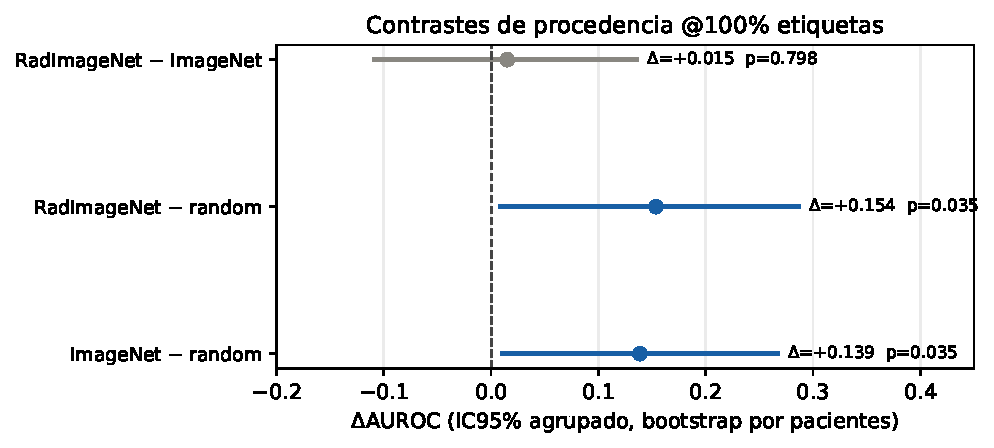
\includegraphics[width=0.95\columnwidth]{fig_forest_delta100}
\caption{Forest plot of paired $\Delta$AUROC at 100\% labels (patient cluster
bootstrap). The RadImageNet$-$ImageNet interval straddles zero; both
pretrained$-$random intervals exclude it. Cohort after QC: 186 patients / 190 knees /
419 views (2 views excluded for image--mask mismatch).}
\label{fig:forest}
\end{figure}

\subsection{Label-efficiency curve and interaction}
Table~\ref{tab:curve} and Fig.~\ref{fig:curve} trace performance as the training-label
budget shrinks. Two facts stand out. First, the RadImageNet$-$ImageNet gap does not
widen as labels become scarce: the per-fraction interaction is
$-0.043$ (10\%), $-0.003$ (25\%), $-0.013$ (50\%), $+0.025$ (100\%), and every 95\%
interval crosses zero ($p$ between 0.53 and 0.99). Provenance never separates.
Second, the benefit of pretraining over random is \emph{concentrated at the full
budget}: at $\le 25\%$ of training patients (13--31 patients) all three
initializations sit near chance, and the pretrained$-$random advantage reaches an
interval excluding zero only at 100\%.

\begin{table}[t]
\caption{Label-efficiency curve (3 seeds; OOF knee-level AUROC, mean $\pm$ SD).
Fractions are nested subsets of \emph{training} patients.}
\label{tab:curve}
\centering
\footnotesize
\setlength{\tabcolsep}{4pt}
\begin{tabular}{lccc}
\toprule
Fraction (train pts.) & RadImageNet & ImageNet & Random \\
\midrule
10\% (13)  & $0.506 \pm 0.022$ & $0.550 \pm 0.045$ & $0.511 \pm 0.024$ \\
25\% (31)  & $0.545 \pm 0.030$ & $0.547 \pm 0.029$ & $0.535 \pm 0.038$ \\
50\% (61)  & $0.621 \pm 0.027$ & $0.634 \pm 0.011$ & $0.544 \pm 0.035$ \\
100\% (122)& $0.688 \pm 0.006$ & $0.663 \pm 0.031$ & $0.526 \pm 0.007$ \\
\bottomrule
\end{tabular}
\end{table}

\begin{figure}[t]
\centering
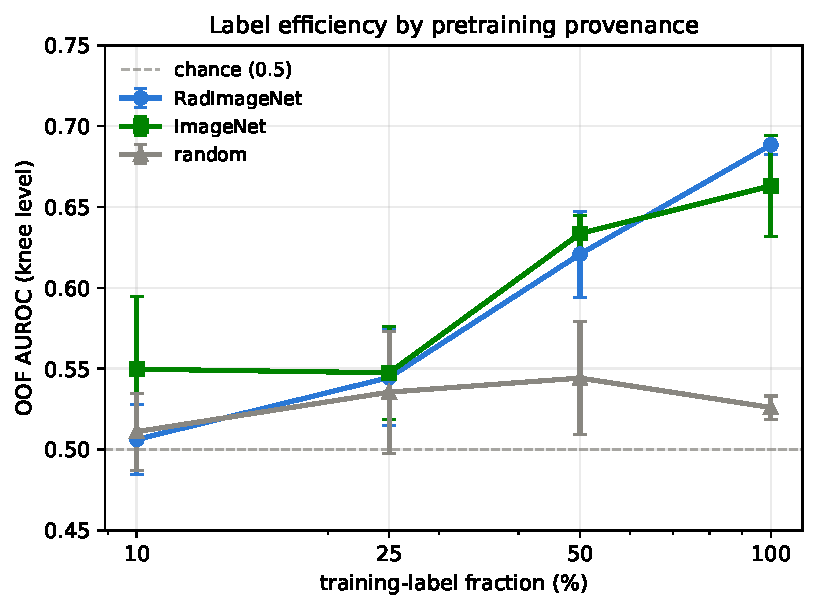
\includegraphics[width=0.95\columnwidth]{fig_efficiency_curve}
\caption{Label-efficiency curve (OOF knee-level AUROC vs.\ training-label fraction; 3
seeds). RadImageNet and ImageNet track each other at every budget; both separate from
random only as the budget approaches 100\%. At $\le 25\%$ all curves sit near the
chance line.}
\label{fig:curve}
\end{figure}

\section{Discussion}
\label{sec:discussion}

\textbf{We did not observe the assumed advantage of radiological pretraining.} Across
five seeds and four label budgets, RadImageNet and ImageNet are indistinguishable at
the knee level in our runs (Tables~\ref{tab:delta100}, \ref{tab:curve}); the point
estimate of their difference is $+0.015$ AUROC with an interval an order of magnitude
wider than the effect. We read this cautiously. It is not evidence against the
neighbouring pipeline, whose contribution is an \emph{unsupervised} phenotype geometry
rather than a predictive comparison~\cite{elnakib26}; at most it invites a second look
at an assumption that recent TPF work adopted from the RadImageNet
literature~\cite{mei22radimagenet}. One plausible reading, consistent with
Transfusion's observation that much of transfer's benefit is low-level rather than
semantic~\cite{raghu19transfusion}, is that if the value of pretraining here is
largely well-scaled early filters, a radiological source need not beat a natural-image
one on a task whose discriminative cue --- cortical disruption around the plateau ---
is a generic edge/texture pattern. We offer this as a conjecture, not a claim.

\textbf{Where pretraining helps reframes what ``label efficiency'' can mean.} The
benefit of any pretraining over random initialization is real but appears only at the
full budget ($\Delta \approx 0.15$, interval excluding zero), and vanishes at
$\le 25\%$, where every initialization --- pretrained or not --- sits near chance
(AUROC $\approx 0.5$). This is the opposite of the pattern one hopes for from
pretraining, which is usually justified precisely by its low-label regime. The most
parsimonious reading is that at 13--31 training patients the bottleneck is not the
\emph{representation} but the \emph{fine-tuning signal}: there are too few labelled
knees for a linear-probe-plus-fine-tune head to locate the decision boundary,
regardless of how the backbone was initialized. ``Label efficiency'' therefore cannot
be claimed for any source here; the honest statement is that pretraining does not
rescue the scarce-label regime for this task, and provenance does not modulate that.

\textbf{Why a modest absolute AUROC does not invalidate the ablation.} Peak AUROC is
$0.68$ --- modest, and we do not present this as a deployable detector. Crucially,
the study's claim is a \emph{contrast}, and the contrast is internally valid: all
three arms share folds, preprocessing, optimizer, augmentation policy, and budget, so
any handicap in the pipeline is applied equally and cancels in $\Delta$AUROC. Two
choices plausibly cap the absolute level --- lighter QC than the eight-step protocol
of~\cite{elnakib26} (we did not exclude wrong-anatomy or post-operative-hardware
cases), and full-frame input without an Otsu-based region-of-interest crop centring
the plateau. Both would be expected to raise the absolute AUROC of \emph{all} arms
together; neither is expected to reverse a provenance ordering whose gap is already
$+0.015$. Establishing that quantitatively --- re-running the ablation on the stricter
cohort with plateau-centred crops --- is the natural robustness check, and we frame it
as future work rather than a threat to the present contrast.

\textbf{A curious next step, held loosely: in-domain self-supervision.} If, in this
preliminary setting, neither natural-image nor general-radiology pretraining
separates from the other, and if pretraining as a class seems to help only once labels
are plentiful, we find ourselves wondering whether the lever worth exploring is a
representation matched to \emph{this} anatomy and modality. Self-supervised objectives
have advanced medical classification when the pretraining distribution is close to the
target~\cite{azizi21,chen20simclr}, and masked-image modelling has shown promising
low-annotation transfer for TPF structures in a different modality~\cite{yue25mae}.
This is precisely the direction of our own thesis work, and these experiments were run
to inform it. Our curve suggests two simple bars an in-domain masked-autoencoder
protocol could be measured against --- whether it beats chance at 10--25\% labels, or
exceeds $0.68$ at 100\%. We put these forward as questions we are curious to answer,
not predictions: it may well be that the limiting factor is the fine-tuning data and
task rather than the representation, and we would want to know that too.

\textbf{Limitations.} The cohort is single-institution, 2D radiography, $n=186$
patients, with no external validation; the absolute AUROC is modest; augmentation and
QC were deliberately conservative; and the curve's low-fraction points rest on 13--31
patients, so their intervals are wide. The findings characterize this task, dataset,
and regime, and should not be read as a general verdict on RadImageNet.

\section{Conclusion}
In this preliminary study, and within its limits, we did not find that pretraining
provenance governs label efficiency for tibial plateau fracture detection: in our runs
RadImageNet showed no detectable advantage over ImageNet at any label budget, and both
exceeded random initialization only once labels were sufficient. We take this
gently, as a working assumption rather than a settled result. For our own immediate
purpose --- designing an in-domain masked-autoencoder perception protocol --- it
suggests, provisionally, that an off-the-shelf ImageNet or RadImageNet initialization
may be treated as interchangeable, which lets us turn our attention to the question we
actually find interesting: whether in-domain self-supervision can move the scarce-label
regime that off-the-shelf transfer, here, left near chance. We hold that as a
hypothesis to verify, not a conclusion, and release fold manifests, out-of-fold
predictions, and configurations so that others --- and our future selves --- can check
and extend it.

\section*{Reproducibility}
Fold manifests, QC exclusion logs, per-run configurations with seeds, out-of-fold
knee-level predictions, and recorded software/hardware versions are released with the
code. Every weight load is guarded by a tensor-count assertion, and zero patient
leakage across folds is enforced by an automated test.

\begin{thebibliography}{99}
\bibitem{vandergaast25} J. van der Gaast \textit{et al.}, ``Deep learning for tibial
plateau fracture detection and classification on plain radiographs,'' \textit{The
Knee}, vol.~54, pp.~81--89, 2025. doi:\,10.1016/j.knee.2025.02.001.
\bibitem{huo25} J. Huo \textit{et al.}, ``Deep learning diagnosis of adult tibial
plateau fractures: a multicentre study with external validation,'' \textit{Radiology
Advances}, vol.~2, no.~3, umaf020, 2025. doi:\,10.1093/radadv/umaf020.
\bibitem{elnakib26} M. Elnakib, M. Saad, and A. Al-Kabbany, ``Phenotyping tibial
plateau fractures via self-supervised learning: a label-agnostic framework with
expert validation,'' arXiv:2606.17295, 2026. doi:\,10.48550/arXiv.2606.17295.
\bibitem{mei22radimagenet} X. Mei \textit{et al.}, ``RadImageNet: an open radiologic
deep learning research dataset for effective transfer learning,'' \textit{Radiology:
Artificial Intelligence}, vol.~4, no.~5, e210315, 2022. doi:\,10.1148/ryai.210315.
\bibitem{raghu19transfusion} M. Raghu, C. Zhang, J. Kleinberg, and S. Bengio,
``Transfusion: understanding transfer learning for medical imaging,'' in \textit{Adv.
Neural Inf. Process. Syst. (NeurIPS)}, 2019. doi:\,10.48550/arXiv.1902.07208.
\bibitem{azizi21} S. Azizi \textit{et al.}, ``Big self-supervised models advance
medical image classification,'' in \textit{Proc. IEEE/CVF Int. Conf. Comput. Vis.
(ICCV)}, 2021, pp.~3478--3488. doi:\,10.1109/ICCV48922.2021.00346.
\bibitem{yue25mae} P. Yue, D. Cai, C. Guo, M. Liu, J. Xia, and Y. Wang, ``Learning
generalizable features for tibial plateau fracture segmentation using masked
autoencoder and limited annotations,'' arXiv:2502.02862, 2025. doi:\,10.48550/arXiv.2502.02862.
\bibitem{chen20simclr} T. Chen, S. Kornblith, M. Norouzi, and G. Hinton, ``A simple
framework for contrastive learning of visual representations,'' in \textit{Proc. Int.
Conf. Mach. Learn. (ICML)}, 2020, pp.~1597--1607. doi:\,10.48550/arXiv.2002.05709.
\bibitem{he16resnet} K. He, X. Zhang, S. Ren, and J. Sun, ``Deep residual learning for
image recognition,'' in \textit{Proc. IEEE Conf. Comput. Vis. Pattern Recognit.
(CVPR)}, 2016, pp.~770--778. doi:\,10.1109/CVPR.2016.90.
\bibitem{rajpurkar18mura} P. Rajpurkar \textit{et al.}, ``MURA: large dataset for
abnormality detection in musculoskeletal radiographs,'' in \textit{Proc. Med. Imaging
Deep Learn. (MIDL)}, 2018. doi:\,10.48550/arXiv.1712.06957.
\bibitem{abedeen23fracatlas} I. Abedeen \textit{et al.}, ``FracAtlas: a dataset for
fracture classification, localization and segmentation of musculoskeletal
radiographs,'' \textit{Scientific Data}, vol.~10, 521, 2023. doi:\,10.1038/s41597-023-02432-4.
\bibitem{thorat24} S. R. Thorat, D. G. Jha, A. K. Sharma, and D. V. Katkar, ``Wrist
fracture detection using self-supervised learning methodology,'' \textit{Journal of
Musculoskeletal Surgery and Research}, vol.~8, no.~2, pp.~133--141, 2024. doi:\,10.25259/JMSR\_260\_2023.
\bibitem{spahr21selftaught} A. Spahr, B. Bozorgtabar, and J.-P. Thiran, ``Self-taught
semi-supervised anomaly detection on upper-limb X-rays,'' in \textit{Proc. IEEE Int.
Symp. Biomed. Imaging (ISBI)}, 2021, pp.~1632--1636. doi:\,10.48550/arXiv.2102.09895.
\bibitem{ssl2tl} F. Hinterwimmer \textit{et al.}, ``From self-supervised learning to
transfer learning with musculoskeletal radiographs,'' \textit{Current Directions in
Biomedical Engineering}, vol.~8, no.~2, pp.~9--12, 2022. doi:\,10.1515/cdbme-2022-1003.
\bibitem{platif26} A. Kazemi \textit{et al.}, ``PlaTiF: a pioneering dataset for
orthopedic insights in AI-powered diagnosis of tibial plateau fractures,''
\textit{Scientific Data}, vol.~13, 240, 2026. doi:\,10.1038/s41597-026-06560-5.
\bibitem{kingma15adam} D. P. Kingma and J. Ba, ``Adam: a method for stochastic
optimization,'' in \textit{Proc. Int. Conf. Learn. Represent. (ICLR)}, 2015. doi:\,10.48550/arXiv.1412.6980.
\end{thebibliography}

\end{document}
